\begin{Exercise}[title=Mesure de la vitesse du son ]
	Le trombone de Koenig est un dispositif de laboratoire permettant de faire interférer deux ondes sonores ayant suivi des chemins différents.
	Le haut-parleur alimenté par un GBF émet un son de fréquence $f=1500$Hz.
	On mesure le signal à la sortie avec un microphone branché sur un oscilloscope. En déplacant la partie mobile $T_1$ on fait varier l'amplitude du sinal observé.
	Elle passe deux fois de suite par une valeur minimale lorsqu'on déplace $T_1$ de $d=11,5cm \pm 2mm$.
	%\begin{figure}[h]
	\begin{center}
		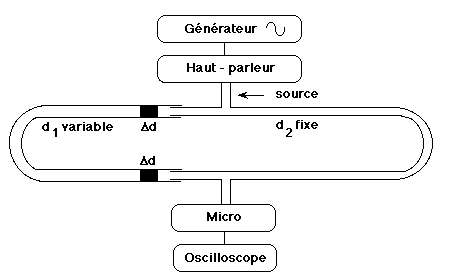
\includegraphics[scale=0.4]{./fig/koenig.jpg}
	\end{center}
	%\end{figure}
	\Question Que se passe-t-il dans le tube?
	\Question Déterminer la vitesse du son --avec incertitude -- dans l'air à \SI{20}{\celsius} température de l'expérience.
\end{Exercise}
\begin{Answer}
	Le micro reçoit deux ondes sonores qui sont passé par les tubes $T_1$ et $T_2$ Ces deux ondes de même fréquence interfèrent.
	Lorsqu'on déplace me tube mobile on fait varier la longueur du trajet de l'onde qui passe par ce tube, modifiant donc le déphasage entre les ondes reçue par le micro.
	Plus précisément lorsqu'on déplace $T_2$ de la distance $d$ vers la gauche on allonge ce trajet de $2d$.
	Le retard temporel par rapport à l'onde passé par $T_1$ augmente de $\frac{2d}{c}$; son retard de phase de $2\pi f \frac{d}{c}$.
	D'autre part l'amplitude détectée par le micro est minimale lorsque les ondes sont en opposition de phase, c'est à dire un retard de phase de $2m\pi + \pi$ où $m \in \N$.
	Entre deux position où l'onde est minimale on a un déphasage de $2\pi$.
	\[ 2\pi f \frac{d}{c} = 2\pi \Rightarrow c=2fd=(345\pm 6 ) m/s\]
\end{Answer}
